\chapter{Analyse spectrale}
\section{Quelles sont les différentes formes physiques utilisées pour le transport de l'information ?}
L'information est véhiculée grâce à un signal physique. Ce signal peut être soit de nature
analogique soit de nature digital (numérique).

Le signal analogique est un signal continu dans le temps. C'est à dire que son amplitude varie
d'une façon continue. Les signaux de notre environnement (voix, image\ldots) sont de nature
analogiques.

\begin{figure}[H]
	\centering
	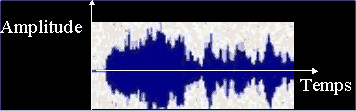
\includegraphics[width=8cm]{partie2/signalanalog.jpg}
\end{figure}

Le signal numérique est un signal discret dans le temps. C'est à dire que son amplitude varie
d'une façon discrète (nombre fini de valeurs). Les signaux générés par certains équipements
(générateurs de tensions électriques ou pulsions) sont de nature numériques.

\begin{figure}[H]
	\centering
	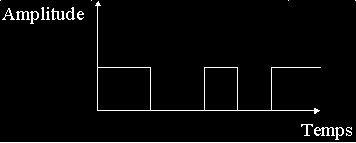
\includegraphics[width=8cm]{partie2/signaldigit.jpg}
\end{figure}
Il ne faut pas confondre l'information avec le signal généré. En effet, l'information utilisée
élémentaire utilisée en informatique est discrète puisque l'ensemble des valeurs est fini
(bit=0 ou 1) tandis que le signal physique le représentant peut être soit numérique soit
analogique. De la même façon qu'on peut véhiculer l'information analogique (par ex.
information vocale) par un signal de nature analogique ou de nature numérique.

\section{Quelles sont les caractéristiques d'un signal analogique élémentaire ?}
Le signal analogique élémentaire est le signal sinusoïdal. C'est un signal périodique
caractérisé par trois paramètres:

\begin{itemize}
	\item La fréquence
	\item L'amplitude
	\item La phase
\end{itemize}
Le signal peut être représenté dans le domaine temporel (amplitude en fonction du temps):
$y(t)=A \sin(2 pft+f)$

Le signal peut être représenté dans le domaine fréquentiel (spectre d'énergie en fonction de
la fréquence). Dans le cas d'un signal sinusoïdal parfait, l'énergie est concentrée sur la
fréquence du signal. Mais le signal durant sa propagation subit des distorsions en fréquence
(comme on le verra plus tard) ce qui conduit à un étalement du spectre autour de la fréquence
théorique.

\section{Comment peut-on caractériser un signal quelconque ?}
Un signal périodique quelconque peut être décomposé en une somme de signaux sinusoïdaux
(Analyse de Fourier).
\begin{figure}[H]
	\centering
	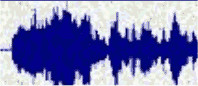
\includegraphics[width=5cm]{partie2/signalaudio.jpg}
\end{figure}

Nous avons alors un spectre de raies. Comme il y a des fluctuations autour de chaque fréquence
contenue dans le signal, nous obtenons un spectre continu. Ainsi, un signal quelconque est
caractérisé par sa bande de fréquences. Plus particulièrement, au niveau quantitatif, nous
nous intéresserons à la largeur de la bande de fréquences.
\begin{figure}[H]
	\centering
	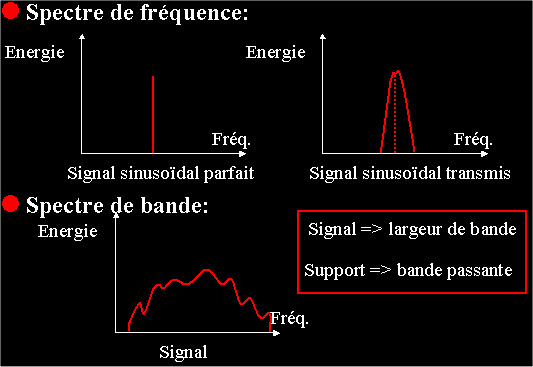
\includegraphics[width=8cm]{partie2/signalfourrier.jpg}
\end{figure}

\section{Quelles sont les déformations affectant un signal ?}
Un signal durant sa transmission subit différentes déformations dues aux caractéristiques du
support de transmission et de l'environnement.

\paragraph{L'affaiblissement} L'affaiblissement d'un signal est du à des caractéristiques du support
(résistance, dispersion de l'onde hertzienne\ldots).

Pour compenser cet affaiblissemnt, on utilise des amplificateurs. L'atténuation (perte) et
l'amplification (gain)s'expriment en décibels (dB): N=10*log10(PS/PE) - le décibel est la
représentation algorithmique d'un rapport de puissances mais on peut l'exprimer avec des
tensions: N=20*log10(TS/TE) avec P=V2/R
PS (resp. TS) et PE (resp. TE) représentent la puissance en sortie (resp. tension en sortie)et
la puissance en entrée (resp. tension en entrée). Pour une perte N est négatif et pour un gain
N est positif.
Le choix de l'échelle logarithmique est du à deux raisons essentielles: la variation de
l'énergie du signal est logarithmique et le fait que des gains et des pertes en cascades se
calculeront par des additions et des soustractions.
On exprime aussi la puissance en dBW: P(dBW)=10*log10P(W) et la tension en dBmV:
T(dBmV)=20*log10T(mV).

\paragraph{Les distorsions} Les distorsions subies par le signal affectent ses paramètres (amplitude,
phase, fréquence). 
La distorsion en amplitude est du au fait que le support a une impédance et pas uniquement une
résistance: l'affaiblissement du signal varie en fonction de la fréquence. Dans ce cas, il
faut utiliser un égalisateur qui amplifie en fonction de la fréquence.
La distorsion en phase est du au fait que la vitesse de propagation varie en fonction de la
fréquence du signal. Dans ce cas, le problème est un problème de synchronisation et nous avons
besoin de solutions de rephasage ou de resynchronisation.
La distorsion en fréquence est du au fait que le support de transmission ainsi que les
équipements d'extrémité filtrent certaines fréquences. Ils sont caractérisés par la bande de
fréquences qu'ils laissent passer ou Bande Passante. Si la Bande Passante n'est pas suffisante
pour la Bande de Fréquences du signal alors il est nécessaire d'effectuer une transmission par
transposition de fréquences.

\paragraph{Les bruits} Un bruit est un signal parasite additif au signal utile. Ce parasitage peut
amener à des erreurs d'interprétation du signal.

Pour limiter au maximum les bruits, différentes techniques sont utilisées agissant sur le type
du support utilisé (coaxial, blindé, torsadé, optique\ldots). L'influence du bruit est mesurée
par le rapport Signal sur Bruit en dB: (S/B)dB = 10*log10(S/B).


\section{Quelle est la capacité d'un support de transmission ?}
La capacité d'un support de transmission est la quantité maximum d'informations qu'il peut
véhiculer par unité de temps. En informatique, cette capacité est exprimée en bits par seconde
(ou ses multiples). Par conséquence, la capacité représente le débit maximum possible ur le
support. Il ne faut pas confondre capacité d'un support et débit d'un équipement. D'après les
travaux de Shannon nous avons: C = W*log2(S/B+1) où C est la capacité en bps, W la largeur de
la bande passante en Hertz et S/B le rapport puissance du signal sur puissance du bruit.



